\documentclass{article}

\usepackage{ctex}

\usepackage{amsmath}
\usepackage{hyperref}
\usepackage{natbib}
\usepackage{graphicx}
\usepackage{minted}
\setminted{breaklines=true, breakanywhere=true, linenos=true}
\usepackage{float}
\usepackage{url}

\title{}
\author{}
\date{}

\begin{document}

\begin{titlepage}
\begin{center}
% \maketitle


\includegraphics[width=0.75\textwidth]{hnu}

\Huge \textbf{创新设计报告}
\vspace{0.5\baselineskip}

\Large
\begin{tabular}{@{}ll}
\textbf{课程名称:} & \underline{\makebox[7cm][c]{电子与计算机系统工程实训}} \\
\textbf{设计项目名称:} & \underline{\makebox[7cm][c]{智能天气显示面板}} \\
\textbf{专业班级:} & \underline{\makebox[7cm][c]{信息安全2101班}} \\
\textbf{姓名:} & \underline{\makebox[7cm][c]{吴\hspace{1em}天}} \\
\textbf{学号:} & \underline{\makebox[7cm][c]{202108060109}} \\
\textbf{指导教师:} & \underline{\makebox[7cm][c]{凌纯清}} \\
\textbf{完成时间:} & \underline{\makebox[7cm][c]{2023年9月6日}} \\
\end{tabular}

\vspace{\baselineskip}
\large 信息科学与工程学院

\end{center}
\end{titlepage}

\clearpage

\begin{abstract}

出门前,经常需要查看今日天气信息决定穿衣、携带雨具等。一般的流程是掏出手机、解锁、找到并打开天气 App、等待开屏广告、向下滑动查看指定信息,这一操作十分繁琐。本装置针对这一细分场景进行优化设计。

本项目产品是一个“智能天气显示面板”,设计该装置安装位置在衣柜或门口处,只需抬眼即可查看到天气,简化查看天气信息的流程,方便用户的出行。装置能够实现与计算机通信、联网查询实时天气,显示室外实时温度(源于网络查询数据)、室内实时温度(源于传感器数据),并显示穿衣和雨具携带建议等功能。

本项目基于STC15F2K60S2开发板,在实现上综合运用了LED数码管、振动传感器、温度传感器、按键、串口通信等多个模块,在STC开发板和计算机上分别编写程序,实现了软硬件的协同设计。

本设计的亮点是,在编写的代码中,定义了“通信协议”的概念,实践和运用了“事件循环”的思想。

\end{abstract}

\clearpage

\tableofcontents

\clearpage

\section{绪论}

\subsection{设计目的}

出门前,经常需要查看今日天气信息决定穿衣、携带雨具等。一般的流程是掏出手机、解锁、找到并打开天气 App、等待开屏广告、向下滑动查看指定信息,这一操作十分繁琐。本装置针对这一细分场景进行优化设计。设计该装置安装位置在衣柜或门口处,只需抬眼即可查看到天气,简化查看天气信息的流程,方便用户的出行。

\subsection{任务与要求}

\begin{itemize}
  \item 主动与计算机通信,通过高德地图API联网查询实时天气。
  \item 将获取到的天气信息在LED数码管上显示。
  \item 通过传感器的数据,显示实时室内温度。
  \item 根据各种数据显示携带雨具等生活建议。
\end{itemize}

\section{系统总体设计}

系统分为STC开发板和计算机两个部分。之间通过串口通信。其中计算机必须能够连接互联网,需要负责向高德地图提供的天气查询API发送请求。整体系统架构图见图\ref{fig:system}。

\begin{figure}[h]
    \centering
    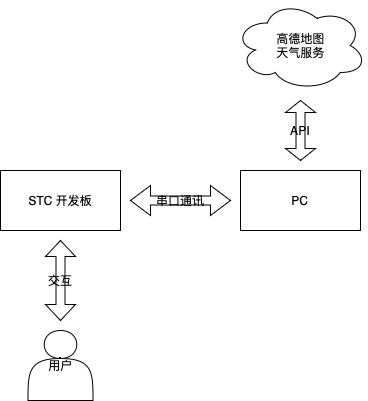
\includegraphics[width=0.5\textwidth]{system}
    \caption{系统总体架构图}
    \label{fig:system}
\end{figure}

\subsection{STC开发板部分}

\begin{itemize}
  \item 检测到振动时,向串口发送天气查询的请求。
  \item 从串口获取请求数据后,更新本地的天气和气温数据。
  \item 按下K1时,显示天气和气温数据。
  \item 按下K2时,显示从传感器获取的温度信息。
  \item 按下K3时,显示携带雨具的建议。
\end{itemize}

\subsection{计算机部分}

\begin{itemize}
  \item 通过独立的配置文件,可以配置所在城市等信息。
  \item 接收到天气查询请求时,向高德地图API发送查询请求,获取返回结果并通过串口发送回开发板。
\end{itemize}

\section{硬件电路原理}

\subsection{开发板整体介绍}

本次使用的 STC 学习板芯片型号为 IAP15F2K61S2,可以通过IAP(应用编程) 或 ISP(系统编程)的方式来将程序烧录到学习板上。

\subsection{各模块原理介绍与电路图}

\paragraph{LED数码管模块}
LED数码管模块由数码管(7段显示器)和LED驱动电路组成。数码管由7个LED段组成,每个段代表数字的一部分。例如,一个7段数码管可以显示0到9的数字以及一些字母。LED驱动电路用来控制这些LED段的亮度和状态。通常,一个数字或字符在数码管上显示时,会将相应的LED段点亮,而其他未用到的段则保持关闭。通过控制每个LED段的状态,可以在数码管上显示各种数字、字符或符号。电路图见图 \ref{fig:led_diagram}。

\begin{figure}[h]
    \centering
    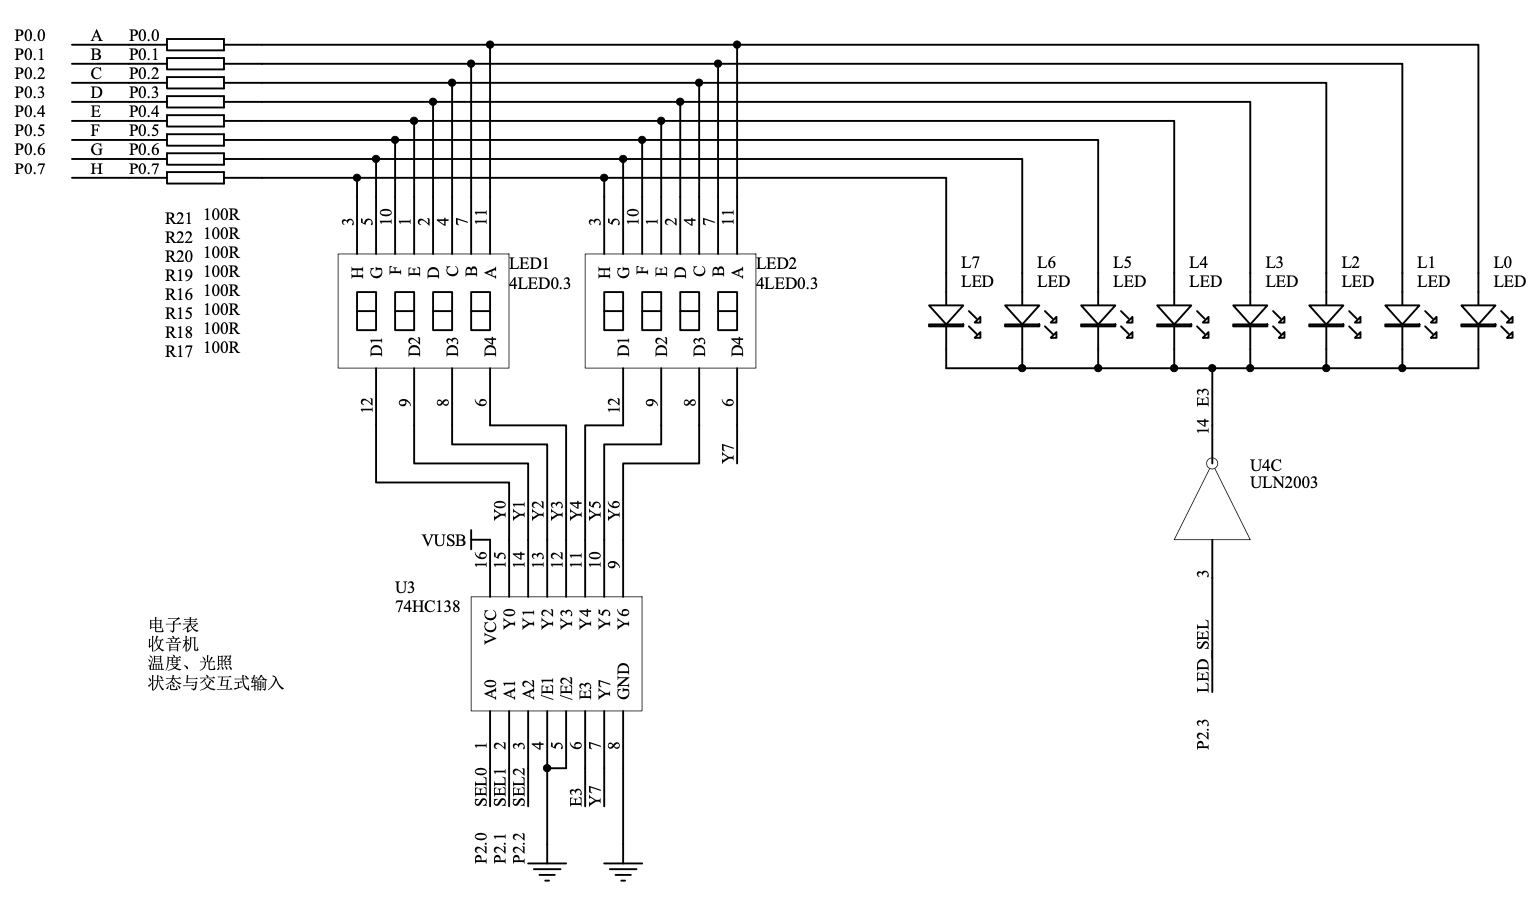
\includegraphics[width=\textwidth]{led_diagram}
    \caption{LED数码管模块电路图}
    \label{fig:led_diagram}
\end{figure}

\paragraph{振动传感器模块}
振动传感器模块用于检测物体的振动或震动。它的基本原理是基于压电效应或加速度测量。一种常见的振动传感器是压电传感器,它包含一个压电晶体材料,当受到振动或压力时,会产生电荷。这个电荷信号被传感器捕获,并转换成与振动幅度和频率相关的电压信号。这个电压信号可以用来检测振动的强度和频率,从而用于各种应用,如震动检测、故障诊断等。电路图见图 \ref{fig:vib_diagram}。

\begin{figure}[h]
    \centering
    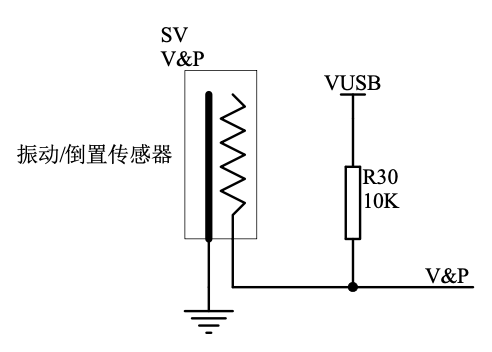
\includegraphics[width=0.25\textwidth]{vib_diagram}
    \caption{振动传感器模块电路图}
    \label{fig:vib_diagram}
\end{figure}

\paragraph{按键模块}
按键模块包括多个按钮,用于用户输入。其基本原理是在按钮被按下时,按钮之间的电接触闭合,导通电流。这个闭合电路的检测可以被连接到微控制器或其他电路中,以检测用户的按键操作。按键模块通常用于用户界面,例如控制面板、键盘或遥控器等。微控制器可以根据按键操作来执行不同的功能,例如启动、停止、选择选项等。电路图见图 \ref{fig:keys_diagram}。

\begin{figure}[h]
    \centering
    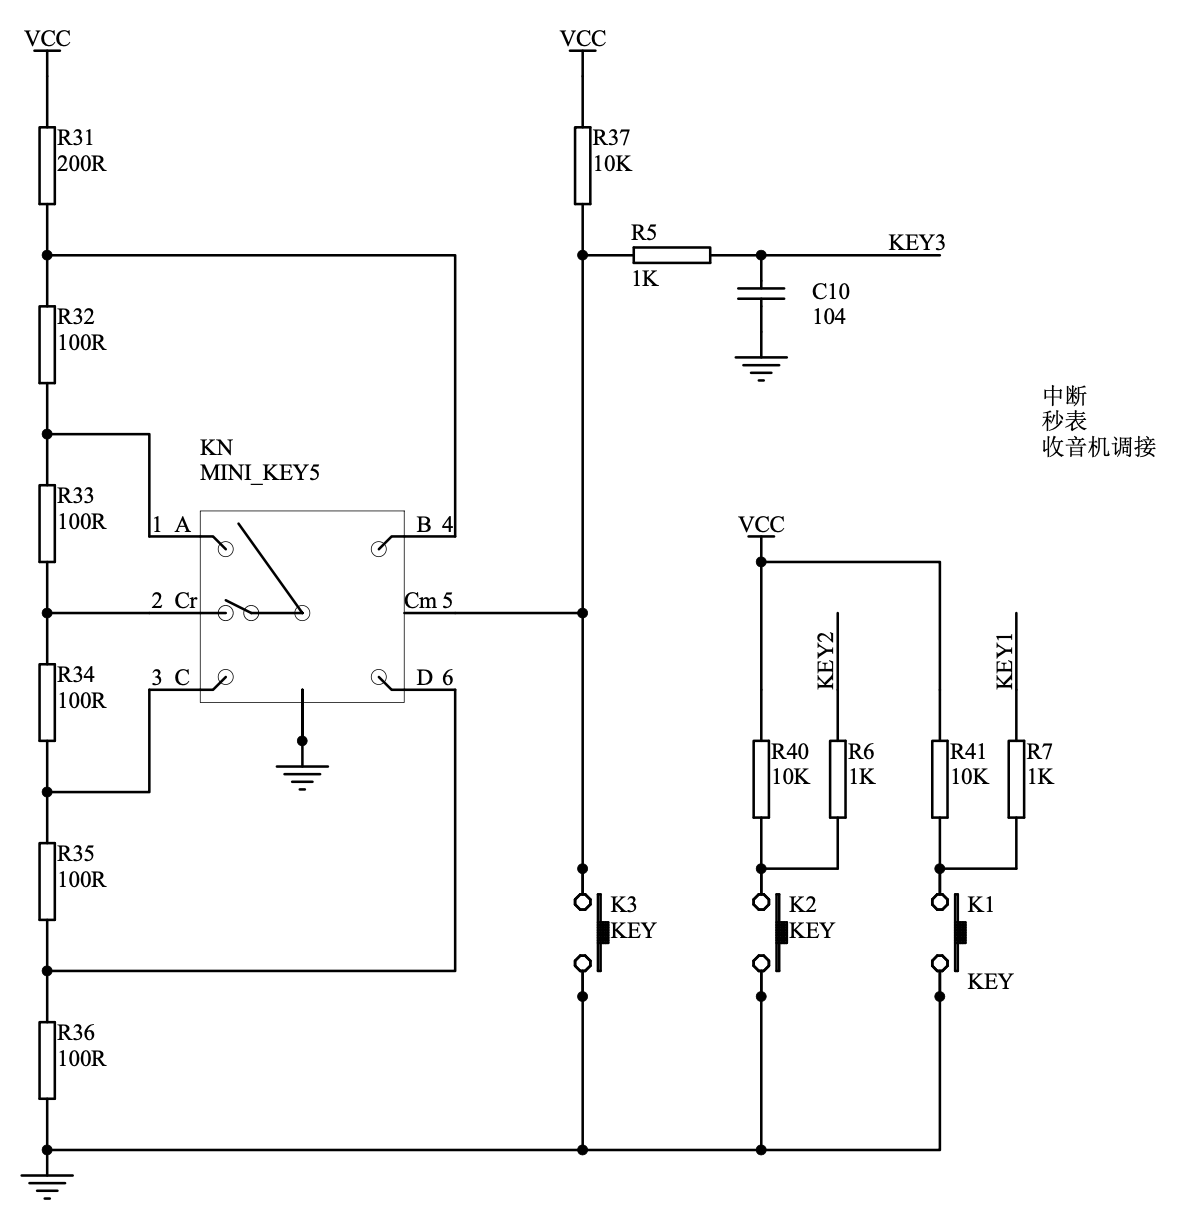
\includegraphics[width=0.75\textwidth]{keys_diagram}
    \caption{按键模块电路图}
    \label{fig:keys_diagram}
\end{figure}

\paragraph{温度传感器模块}
温度传感器模块使用热敏电阻来测量环境温度。热敏电阻是一种电阻随温度变化而变化的元件,其基本原理是电阻与温度成反比例关系。当温度升高时,热敏电阻的电阻值减小,反之亦然。通过测量电阻值的变化,可以确定当前的温度。温度传感器模块通常将热敏电阻连接到一个电路中,并使用微控制器或模拟电路来读取电阻值并将其转换为温度值。这样的模块在温度监测和控制应用中非常常见,例如室内温度控制、温度报警系统等。电路图见图 \ref{fig:rt_diagram}。

\begin{figure}[h]
    \centering
    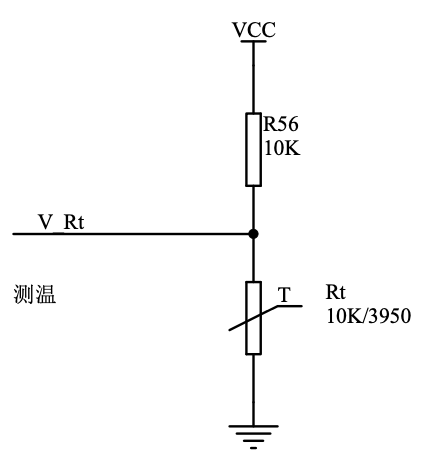
\includegraphics[width=0.25\textwidth]{rt_diagram}
    \caption{温度传感器模块电路图}
    \label{fig:rt_diagram}
\end{figure}

\paragraph{串口通信模块}
串口通信模块是一种用于在设备之间进行数据传输的通信接口。其基本原理涉及到将数据序列化为一系列比特,然后通过串行方式将这些比特逐个传输。通常,串口通信模块包括两个主要线路:发送线路(TX)和接收线路(RX)。发送设备将数据通过TX线发送,接收设备通过RX线接收数据。在STC开发板中,此模块是UART通信接口,集成于mini USB接口。电路图见图 \ref{fig:serial_diagram}。

\begin{figure}[h]
    \centering
    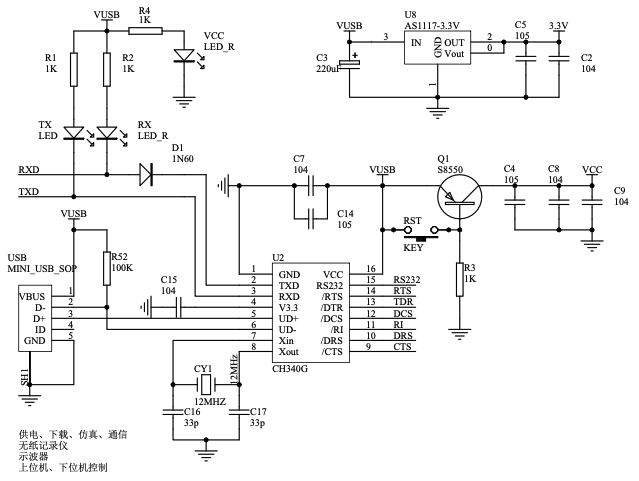
\includegraphics[width=0.9\textwidth]{serial_diagram}
    \caption{串口通信模块电路图}
    \label{fig:serial_diagram}
\end{figure}

\section{软件设计与实现}

在构建本系统时,编写的软件,主要包括两部分:STC开发板上刷入运行的程序,以及计算机上运行的程序。两个程序之间通过串口通信。

\subsection{交互协议约定}

STC与PC之间通过串口发送的数据交互,需要约定一套数据语义(即“协议”)。在本系统中,约定:

\begin{itemize}
  \item 一个“数据包”长度为5字节,并以 0xAA 0x55 开头。
  \item 一个“查询数据包”内容是 0xAA 0x55 0xFF 0xFF 0xFF。
  \item 一个“响应数据包”内容形如 0xAA 0x55 X Y Z,其中:
  \begin{itemize}
    \item X 为天气,可以为 0x00、0x01、0x02 或 0x03,分别表示晴天、多云、雨、雪。
    \item Y 为温度数据,表示为一个 8 位有符号整数(即 signed char)。
    \item Z 为保留字节,可以为任意值。这一字节可以在之后扩展其他功能。
  \end{itemize}
\end{itemize}

\subsection{STC开发板部分}

\subsubsection{软件设计}

STC开发板部分的程序直接与用户进行交互,并通过串口与计算机交互。

本程序基于BSP编写。其代码流程图如图\ref{fig:stc_flow}。

\begin{figure}[h]
    \centering
    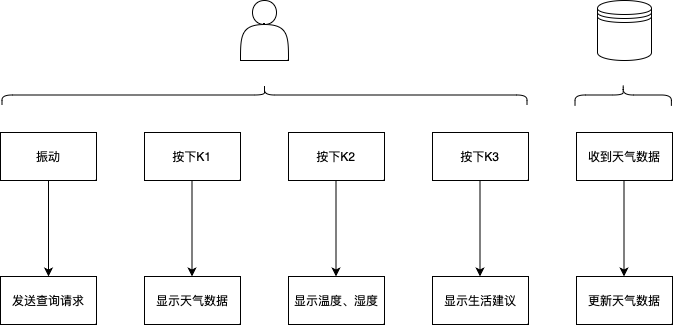
\includegraphics[width=1\textwidth]{stc_flow}
    \caption{STC开发板程序流程图}
    \label{fig:stc_flow}
\end{figure}

代码的主要逻辑基于“事件循环”,由五种事件绑定五种不同的回调函数,以实现程序功能。

\subsubsection{核心函数代码实现}

\paragraph{常量与全局变量} 代码开头定义了常量数组 decode\_table,这是用于 LED 数码管显示的编码表。除了 0 至 9 的数字以及 10 号空白之外,从 11 开始定义了各个所需字母、字符的显示。代码如下:

\begin{minted}{cpp}
code char decode_table[] = {
  0x3f,0x06,0x5b,0x4f,0x66,0x6d,0x7d,0x07,0x7f,0x6f,
  0x00,0x6d,0x1c,0x54,0x39,0x38,0x5c,0x5e,0x50,0x77,0x04,0x79,0x80,0x40};
/*
  10 (empty)
  11 S
  12 u
  13 n
  14 C
  15 L
  16 o
  17 d
  18 r
  19 A
  20 i
  21 E
  22 .
  23 -
  */
\end{minted}

定义天气代码有4种,从0到3分别是晴、多云、雨、雪。定义全局常量 weat2code\_table 码表,在其中定义各个代码对应的英文字母的数码管显示,方便之后使用。同时定义了 Error 和省略号的数码管显示备用。

\begin{minted}{cpp}
code char weat2code_table[6][5] = {
  {11, 12, 13, 10, 10}, // Sun
  {14, 15, 16, 12, 17}, // CLoud
  {18, 19, 20, 13, 10}, // rAin
  {11, 13, 16, 12, 10}, // Snou
  {21, 18, 18, 16, 18}, // Error
  {22, 22, 22, 22, 22}  // ..... (waiting for sync)
};
\end{minted}

全局变量 buf 存放LED数码管显示的内容。本设计中 K1、K2、K3 对应三个不同功能模块,故数码管对应三个部分的不同显示,将其分别存储。全局变量 show 指示当前显示的功能模块。

\begin{minted}{cpp}
char buf[3][8] = {
  {22,22,22,22,22,10,22,22},
  {10,10,10,10,10,10,22,22},
  {10,10,10,10,10,10,10,22}
};

char show = 0;
\end{minted}

定义全局常量 req(即 request)表示发送数据包的内容。

\begin{minted}{cpp}
char req[5] = {0xaa,0x55,0xff,0xff,0xff};
\end{minted}

\paragraph{主函数 main} 基于“事件循环”的思想,主函数中只进行各种模块的初始化,以及事件与回调函数的绑定。在主函数中没有实际上的业务代码。

\begin{minted}{cpp}
void main()
{
  VibInit();
  Uart1Init(2400);
  DisplayerInit();
  SetDisplayerArea(0,7);
  KeyInit();
  AdcInit(ADCexpEXT);

  SetUart1Rxd(rxd, 5, matchhead, 2);
  SetEventCallBack(enumEventUart1Rxd, uart1rxd_callback);
  SetEventCallBack(enumEventSys100mS, sys100ms_callback);
  SetEventCallBack(enumEventSys1mS, sys1ms_callback);
  SetEventCallBack(enumEventVib, vib_callback);
  SetEventCallBack(enumEventKey, key_callback);
  SetEventCallBack(enumEventNav, nav_callback);

  MySTC_Init();
  while (1) MySTC_OS();
}
\end{minted}

\paragraph{100ms 时钟回调函数} 代码中绑定了100ms的时钟回调函数,每100ms会调用一次。此函数只需用于维持LED数码管的显示。buf 和 show 变量的定义如前所述。

\begin{minted}{cpp}
void sys100ms_callback(){
  Seg7Print(buf[show][0],buf[show][1],buf[show][2],buf[show][3],buf[show][4],buf[show][5],buf[show][6],buf[show][7]);
}
\end{minted}

\paragraph{1ms 时钟回调函数} 代码绑定的 1ms 时钟回调函数,主要用于更新温度。由于温度传感器(热敏电阻)得到的数据需要在一段时间内累计取平均值并更新,需要计数器 t 和 sumt 辅助计算温度。

\begin{minted}{cpp}
void sys1ms_callback(){
  t++;
  if (t == 200){
    set_buf_temp(1, tempdata[(sumt+t/2)/t - 1]);
    sumt = t = 0;
  }
  adc_data = GetADC();
  sumt += adc_data.Rt >> 2;
}
\end{minted}

\paragraph{数据更新函数} 代码中定义了 update\_data 函数,这一函数用于向PC发送请求数据包。当收到返回的数据包时,触发 uart1rxd\_callback 回调函数,对天气数据、温度数据、雨具建议进行更新。

\begin{minted}{cpp}
void set_buf_weat(char weat){
  int i;
  if (weat > 3){
    set_buf_error();
    return;
  }
  for (i=0;i<5;i++) buf[0][i] = weat2code_table[weat][i];
}

void set_buf_temp(int target, signed char temp){
  if (temp < 0) buf[target][5] = 23, temp=-temp;
  buf[target][6] = temp/10 % 10;
  buf[target][7] = temp % 10;
}

void set_buf_rg(char f){ // rain gear
  buf[2][7] = f?18:16;
}

void update_data(){
  Uart1Print(req, 5); // send request
}

void uart1rxd_callback(){
  set_buf_weat(rxd[2]);
  set_buf_temp(0,rxd[3]);
  
  set_buf_rg(rxd[2] == 2 || rxd[2] == 3);
}
\end{minted}

\paragraph{按键响应函数} 开发板上的 K1、K2、K3 按键按下时,应该能够切换 LED 显示的不同内容,即切换 show 全局变量的值。当按下按键时,触发回调函数 key\_callback。需要注意的是,对于 K3,由于使用了ADC模块,必须单独在导航键的回调函数中判断。

\begin{minted}{cpp}
void key_callback(){
  if (GetKeyAct(enumKey1) == enumKeyRelease){
    show = 0;
  }
  if (GetKeyAct(enumKey2) == enumKeyRelease){
    show = 1;
  }
}

void nav_callback(){
  if (GetAdcNavAct(enumAdcNavKey3) == enumKeyRelease){
    show = 2;
  }
}
\end{minted}

\paragraph{振动传感器回调函数} 当振动传感器监测到振动,会触发其回调函数。在回调函数中我们发送请求更新数据。

\begin{minted}{cpp}
void vib_callback(){
  char vib_act = GetVibAct();
  if (vib_act == enumVibQuake) update_data();
}
\end{minted}

\subsection{计算机部分}

\subsubsection{软件设计}

计算机部分的程序主要通过串口与STC开发板交互,并通过高德地图提供的API查询天气信息。

本程序使用 Python 编写。其代码流程如图\ref{fig:pc_flow}。

\begin{figure}[h]
    \centering
    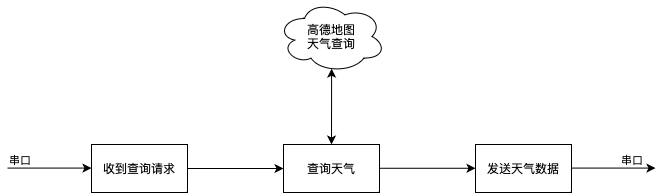
\includegraphics[width=1\textwidth]{pc_flow}
    \caption{计算机程序流程图}
    \label{fig:pc_flow}
\end{figure}

代码对串口进行持续监听,如果串口发送了查询请求,则程序向高德地图API查询天气,并将数据发送给串口。

\subsubsection{核心函数代码实现}

\paragraph{天气查询函数}

代码中的天气查询函数 get\_weather 如下:

\begin{minted}{python}
def get_weather():
    url = f"https://restapi.amap.com/v3/weather/weatherInfo?key={api_key}&city={city_code}&extensions=base"
    try:
        response = requests.get(url)
        if (response.status_code == 200):
            data = json.loads(response.text)
            print(data)
            print(data["lives"][0]["weather"])
            print(data["lives"][0]["temperature"])
            # ref: https://lbs.amap.com/api/webservice/guide/tools/weather-code/
            weat = get_weather_code(data["lives"][0]["weather"])
            temp = data["lives"][0]["temperature"]
        else:
            print(f"ERROR: status code not 200")
    except requests.exceptions.RequestException as e:
        print(f"Exception: {e}")
\end{minted}

这段代码首先构造出请求 URL,然后使用 Python 的 requests 库发送请求。解析请求返回的 json 格式数据,从中提取我们需要的天气信息,并打印、存入变量。

如果 HTTP 响应码不是 200,或者出现了其他异常,程序都会抛出异常。

\paragraph{监听、发送数据函数}

代码中的监听、发送数据函数 listen\_device 如下:

\begin{minted}{python}
def listen_device():
    try:
        ser = serial.Serial(port, baudrate, timeout=timeout)
        if ser.is_open:
            print(f"Opened {port}, Listening...")

            buf = bytes([])
            while True:
                buf = buf + ser.read(1)
                if is_request(buf):
                    print("Request received")
                    buf = bytes([])

                    get_weather()
                    data_to_send = bytes([0xAA, 0x55, weat, temp, 0x00])

                    ser.write(data_to_send)
                    print(f"Data sent: {data_to_send.hex()}")
        else:
            print(f"Unable to open the port {port}")
    except serial.SerialException as e:
        print(f"Serial exception:: {e}")
    except Exception as e:
        print(f"Other exception: {e}")
    finally:
        if ser.is_open:
            ser.close()
            print(f"Closed {port}")
\end{minted}

这段代码首先打开串口开始监听,然后使用 while 循环持续读取串口中传输的字节,存入缓冲区。使用 is\_request 判断是否形成了一个请求数据包,如果是则查询天气、向串口发送查询结果数据包。

如果开启串口失败或者在程序运行过程中出现任何异常,则立即抛出异常。在结束程序时,关闭串口。

\paragraph{配置文件} 为了方便不同用户的使用,代码将不同用户的个性信息存储为独立于代码的配置文件,践行“代码与数据分离”的原则。配置信息包括:所在城市代码、高德地图 API Key、串口名称。使用 Python 的 configparser 库读取和解析独立的配置文件。

\begin{minted}{python}
import configparser

conf = configparser.ConfigParser()
conf.read('config.ini')
port = conf['serial']['port']
api_key = conf['api']['api_key']
city_code = conf['api']['city_code']
\end{minted}

配置文件示例如下:

\begin{minted}{python}
[serial]
port = /dev/tty.usbserial-1140

[api]
api_key = 3e61ddd4ee6d9dd09f55f3f111119cf65
city_code = 430104
\end{minted}

其中城市编码(city\_code)可以参考高德地图接口文档提供的《城市编码表》:\url{https://lbs.amap.com/api/webservice/download}。

\section{系统测试与分析}

\subsection{测试环境介绍}

\begin{itemize}
  \item 测试时间:2023年9月6日
  \item 测试地点:湖南省长沙市岳麓区(当日天气:晴,33 度)
  \item PC 设备:MacBook Air M1,2020
  \item 操作系统:macOS Sonoma
  \item 软件环境:Python 3.9.7
\end{itemize}

\subsection{测试结果分析}

将开发板连接PC通电后,LED 屏幕显示省略号,表示等待数据更新。

运行PC上的Python程序,摇动开发板或轻按振动传感器,PC显示数据查询的输出(见图\ref{fig:test_screenshot}),开发板LED更新信息,显示为”Sun 33“,表示晴,33摄氏度。

按下K2,LED 显示 29,表示传感器检测到室内温度29度。

按下K3,LED 显示“o”,表示不需携带雨具。如果需要携带雨具则会显示为“r”。

按下K1,LED 显示“Sun 33”,回到初始显示状态。

\begin{figure}[h]
    \centering
    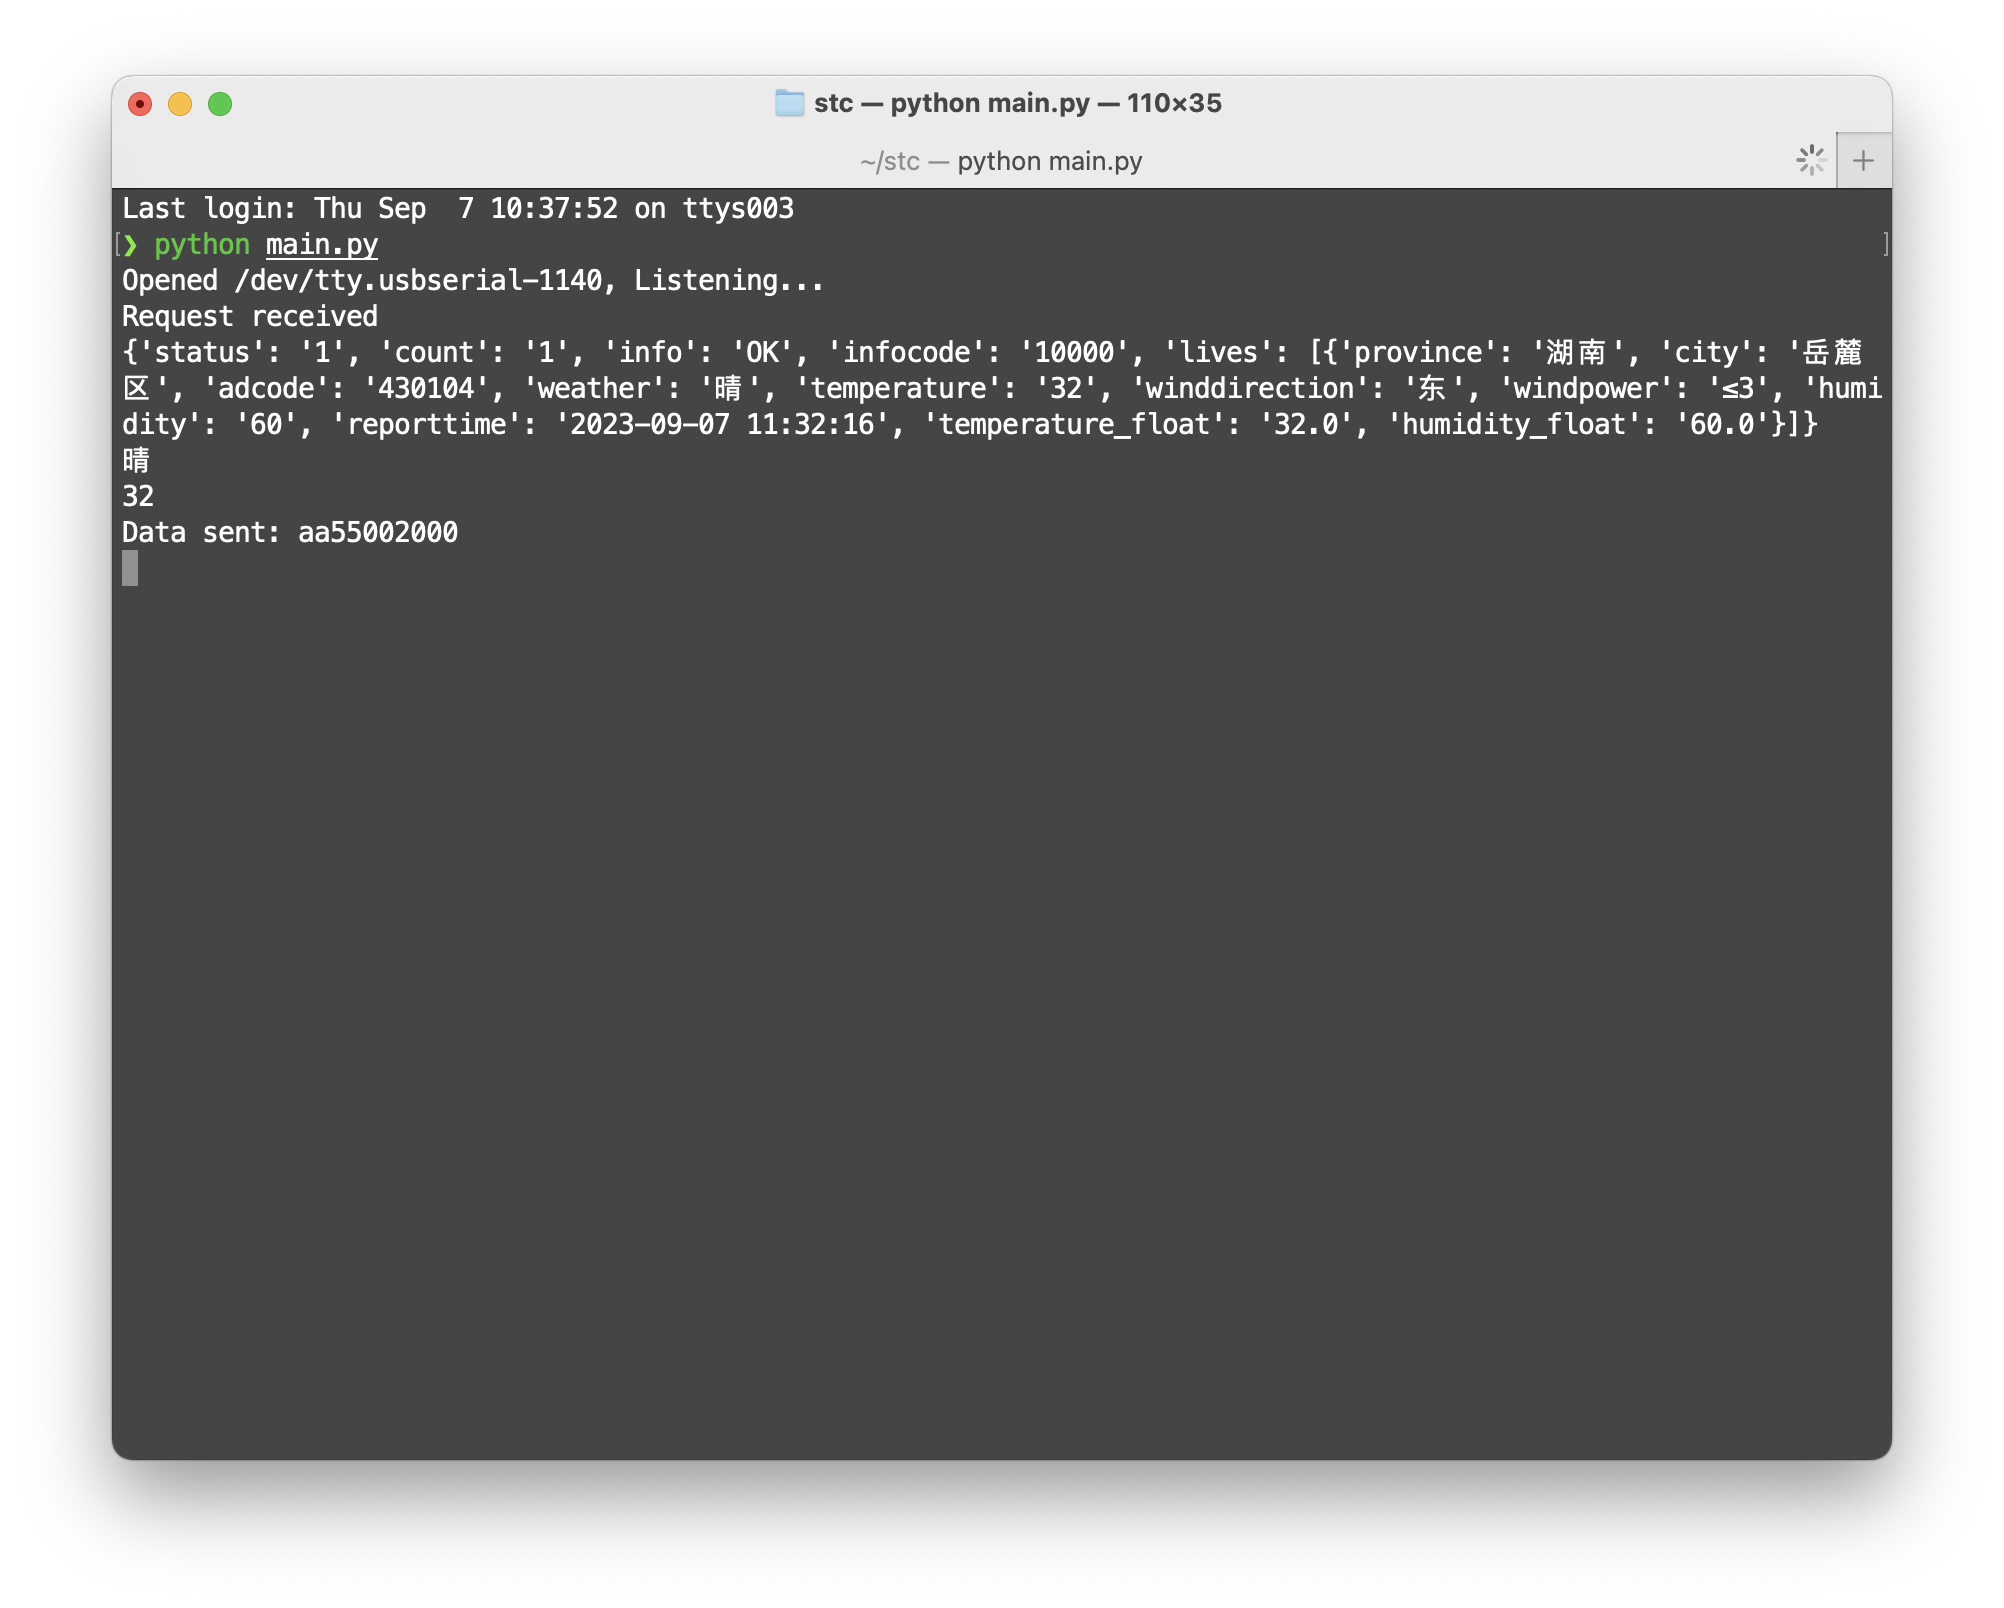
\includegraphics[width=1\textwidth]{test_screenshot.png}
    \caption{PC上运行的程序输出截图}
    \label{fig:test_screenshot}
\end{figure}

\section{结论}

\subsection{成功实现的功能}

\begin{itemize}
  \item 主动与计算机通信,通过高德地图API联网查询实时天气。
  \item 将获取到的天气信息在LED数码管上显示。
  \item 通过传感器的数据,显示实时室内温度。
  \item 根据各种数据显示携带雨具等生活建议。
\end{itemize}

\subsection{收获与感想}

本项目设计基于STC开发板,综合应用了LED显示模块、温度传感器、振动传感器、串口通信模块等多个模块的功能,实现了本项目的综合设计。在学习和设计的过程中,我们对嵌入式开发、软硬件的协同都有了更加深刻的理解和体会。

本设计的与众不同之处是对于“通信协议”概念的设计。在串口通信中,将特定格式的字节流抽象为“数据包”,并分为“查询数据包”和“返回数据包”,这种“约定”可以视为一种“协议”。本设计约定的协议具有可拓展性,可以在传输可靠性等方面进行改进(详见下文“不足之处”)。通过这种设计和实现,我们对通信与通信协议有了更加深刻的理解。

本设计的另一大特点是对于“事件驱动模型”的应用。这一思想来源于操作系统,也在诸如 Node.js 等先进的开发技术上得到了大量应用。具体来说,本设计中编写的所有程序不同于往常的顺序执行,而是将特定事件与其回调函数绑定,使事件触发回调函数执行。徐成老师编写的开发板操作系统BSP本身基于此设计;在本人自己编写的 Python 代码中,则使用永远执行的while循环来模拟“事件驱动模型”。通过本次项目编写的实践,我们对“事件驱动模型”有了更加深刻的理解。

\subsection{不足之处}

由于本人在夏季小学期后半程担任辅导员助理,参与学校迎新工作,故完成此设计的时间有限。该设计的功能仍有大量可改进空间。

\paragraph{可靠传输协议的设计} 在串口传输过程中,容易产生数据差错。在本系统的设计中,传输完成后协议并没有提供确认(ACK)。如果数据产生差错,协议并没有设计纠错或重传机制。结合上学期修读的《计算机网络》课程的相关知识,我们可以模仿TCP等网络传输协议,在不可靠环境中设计一个可靠传输协议。

\paragraph{显示方式的扩展} 使用LED数码管难以直观显示英文(如 rain 只能显示为 rAin,Snow 只能显示为 Snou),和人的信息交互还存在可以改进的空间。可行的改进措施是外接精度更高的数码管,或者外接显示屏。

\paragraph{功能的扩展} 在传输协议中,发送的“相应数据包”保留了一个未使用的字节。如果需要继续改进、添加更多功能,可以使用这个字节携带数据。

\section{参考文献}

\begin{enumerate}
  \item STC-B学习板原理图(教师提供)。
  \item STC-B学习板提供的案例实验、工程文件(教师提供)。
  \item BSP 库文件 sys.h、uart1.h、displayer.h、sys.H、Vib.h、Key.H、adc.h 等文件中的注释说明(教师提供)。
  \item 高德天气查询接口文档:\url{https://lbs.amap.com/api/webservice/guide/api/weatherinfo}。
  \item 高德地图《城市编码表》:\url{https://a.amap.com/lbs/static/amap_3dmap_lite/AMap_adcode_citycode.zip}
\end{enumerate}

\end{document}